\section{Design}
\subsection{Design Overview}
The design is split into a number of sections.Firstly I detail the software components that make up the overall system. Then I go in to detail more detail on each component. We start with the Honeypot application that finds and attacks vulnerable devices, and then move on to looking at the structure of the leaky Android application and how to overcome the problem of using platform specific code within the game, then look at the server application. 
\subsection{Overall System Architecture}
The scenario that this project hypothetically aims to work in is in an area with high traffic, such as a Student Union bar, or a busy public transport station. In reality the applications are designed to meet the ethical guidelines set forth at the beginning of the project whereby a user's consent must be gained prior to taking place in any experimentation. Due to this restriction care must be taken within the design to ensure, where appropriate, devices are filtered and ignored on a set of criteria. This criteria may be MAC address of devices broadcasting probe requests or the SSID present in probe requests. As set out in the requirements the filter will be based on the latter of the two proposed, filtering devices based on the SSID they are probing for. In doing so removes the limitation of testing one device at a time- theoretically having to update the MAC address filter for each new device- and allows us to connect multiple devices running different operating systems at the same time to determine the effectiveness of the overall implementation of the honeypot attack. It should be noted that the leaky application, designed to demonstrate the ease in which applications can broadcast personal data unencrypted, will only be available on Android due to the relative simplicity in creating an application for the environment, and availability of devices. 

\begin{figure}[h!]
\centering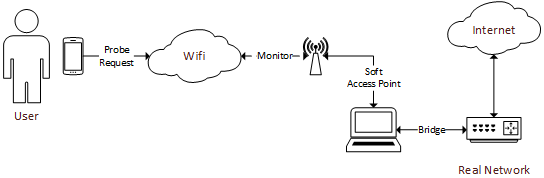
\includegraphics[width=\linewidth]{design/figures/overall.png}
\caption{Overall system architecture.}
\end{figure}

A soft access point is created on the detection of a valid probe request, which is defined as being a request from a device that is looking to reconnect to a network with no authentication method, and the network traffic is then bridged to an actual network to ensure that the user is still able to access the internet, and the attacker can monitor passing traffic.

\subsection{Honeypot}
\subsubsection{High Level Program Flow}
\label{program-flow}
Figure \ref{fig:honeypot_flow} details the high level application flow for the honeypot program. 

\begin{figure}[h!]
\centering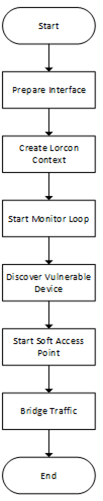
\includegraphics{design/figures/honeypot-flow.png}
\caption{Overall system flow.}
\label{fig:honeypot_flow}
\end{figure}

The application needs to start by creating an interface that is able to capture and inject packets, as this is required by Lorcon to create the context for the packet capture loop. Once setup the monitor loop can begin to parse captured packets until it finds a vulnerable device, after which the application spawns a fake access point and bridges the traffic.
\newpage
\subsubsection{Parsing Probe Request Frames}
\label{parsing-probe}
One of the requirements is to ensure that the SSID that the application looks for can be defined by the user. This argument defined on the command line is then taken by the application and used when parsing probe request frames, as detailed in figure \ref{fig:ssid-machine}

\begin{figure}[h!]
\centering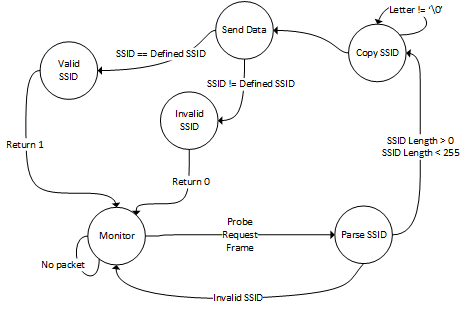
\includegraphics{design/figures/valid-ssid.png}
\caption{Probe request frame parser state machine.}
\label{fig:ssid-machine}
\end{figure}

The application firstly needs to find out whether the SSID is hidden, by checking if the length field in the header is 0, or invalid, by checking if the same field is greater than 255. If it is a valid SSID, it copies the SSID value from the packet header and compares it against the defined SSID from the user, then returns a value to the monitor loop. Also included is the TCP client sending data to the server each time it receives a valid SSID. 

\subsubsection{Discovering Vulnerable Devices}
\label{open-auth}
Figure \ref{fig:discover_device_seq} details the process in which the application goes through to discover a vulnerable device. It parses frame types until it finds a probe request, parses that request as defined in section \ref{parsing-probe}, then sending a response to trigger an association request from the device so it can determine the authentication type that the previous access point used. If it was an open access point that the device had previously connected to it returns a success value and allows the application to move on to the next  stage of the attack, creating the fake access point.
\clearpage
\begin{figure}[h!]
\centering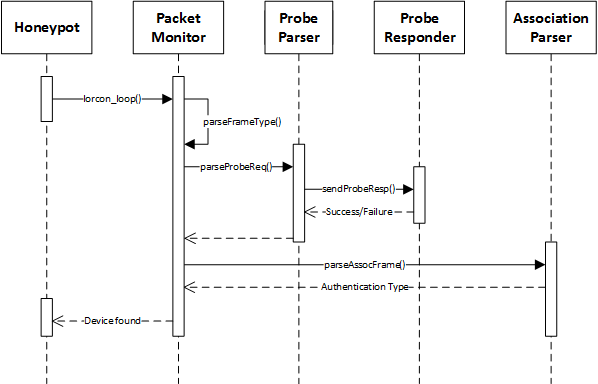
\includegraphics[width=\linewidth]{design/figures/discover-device-seq.png}
\caption{Discovering vulnerable device sequence.}
\label{fig:discover_device_seq}
\end{figure}

\subsubsection{Creating a Fake Access Point}
\label{design:create-ap}
The fake access point shall be created by forking the application and running Airbase-ng, as this is the quickest and most reliable way to achieve what is needed. Writing my own access point, whilst interesting, is not the goal of this project. Using Airbase to create a fake access point is covered in section \ref{sec:spoofap} on page \pageref{sec:spoofap}.


\subsubsection{TCP Client}
\label{hp-tcp}
As the honeypot application is required to collect data about probe requests being broadcasted, a simple TCP client is required to send data to the server. The data to be captured is as follows:

\begin{enumerate}
\item MAC address of the device
\item SSID the device is looking for
\end{enumerate}

Due to the simple nature of this the application will concatenate the two string values using a delimiter to enable the server to easily tokenise and parse the message. In this case I have opted to use a comma as the delimiter, giving the message this structure:

\begin{verbatim}
00:de:ad:00:be:ef,Wireless Lab
\end{verbatim}

As we cannot guarentee the server will be active at all times, the client must connect and disconnect each time it attempts to send data, as detailed in figure \ref{fig:hp_tcp_server}. 

\begin{figure}[h!]
\centering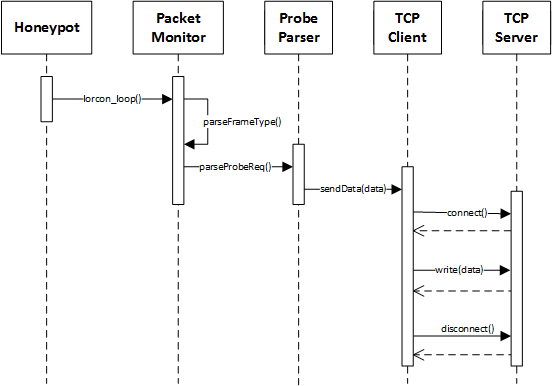
\includegraphics[width=\linewidth]{design/figures/hp-tcp-client.png}
\caption{TCP client/server interaction.}
\label{fig:hp_tcp_server}
\end{figure}

\clearpage
\subsection{Android Game}
\subsubsection{Flappy Bird}
\label{design:flappy-bird}
I have chosen to clone a recently popular game, that has seen an increase of clones in the past few months, Flappy Bird. The reason for chosing this is the simplicity of the overall game, and the virality that it has displayed. This version will be named Leaky Bird to reflect it's actual purpose of leaking data, not being fun. 

\begin{figure}[h!]
\centering
\includegraphics{design/figures/flappy-b-1.png}
\caption{Flappy Bird's simple instructions.}
\label{fig:android_fb1}
\end{figure}

The premise behind Flappy Bird is simple, the player needs to tap the screen in order to make the bird rise and go through a pair of gates, in the form of pipes. Each time the player successfully maneuvers through a set of obstacles the player is awarded a point.

The total points are recorded, and the top three recorded in the high scores. The artwork from the game was borrowed from a well known game publisher, Nintendo, who used similar sprites in their Mario titles.

\subsubsection{Leaky Bird Sprite Sheet}
As the game is not the main focus of this report, and is a clone of an existing game, a sprite sheet will be used that consists of the original artwork, pictured in figure \ref{fig:leaky-spritesheet} on page \pageref{fig:leaky-spritesheet} in the Appendix. This spritesheet will be split in to separate images by the game.

\clearpage
\subsubsection{Leaky Bird Class Diagram}
The Leaky Bird game design, similar to it's parent game,  is relatively simple. It consists of two main classes that inherit from the libgdx screen class, with the GameScreen class holding the GameRenderer and GameWorld which renders and holds the game state respectively doing the majority of the work.

\begin{figure}[h!]
\centering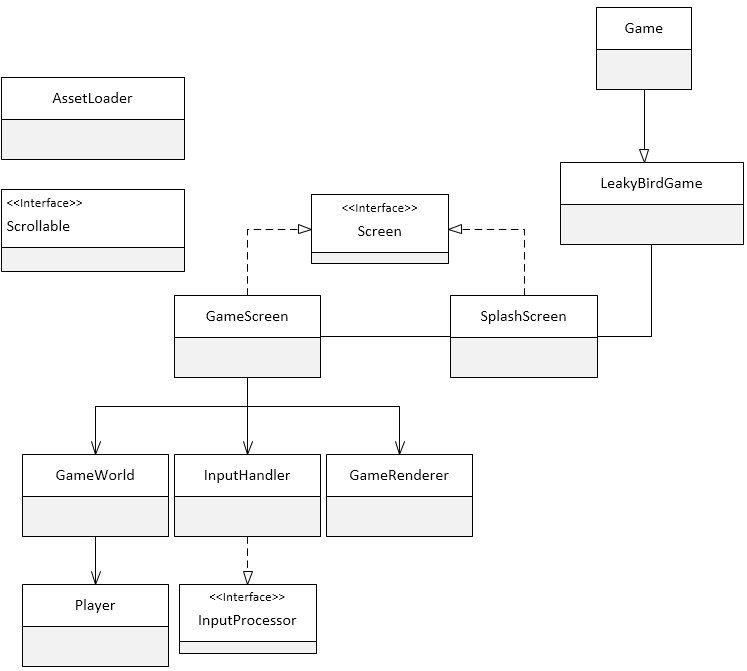
\includegraphics[width=\linewidth]{design/figures/ag-cd.png}
\caption{Android game class diagram.}
\end{figure}
\clearpage
\subsubsection{Android Location Provider}
\label{design:ag-lp-cd}
To successfully use platform specific functionality within the libgdx game environment an interface needs to be created to allow use of the functions. More detail on this can be found in the implementation section; however, figure \ref{alp-class} details the classes required to provide the game with the ability to get location information from the Android device.

\begin{figure}[h!]
\centering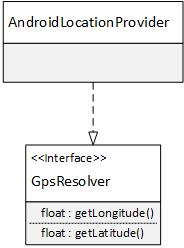
\includegraphics{design/figures/ag-lp-cd.png}
\caption{Android Location Provider class.}
\label{alp-class}
\end{figure}

\subsubsection{TCP Client Provider}
\label{design:ag-tcp-1}
Android applications require any network communications to be performed on a separate thread to that which the UI is currently running on. This stops the application from becoming unresponsive during long connection times or heavy data transfers. As a result of this the TCP client connection, data transfer, and disconnection must run on an AsyncTask when executed otherwise the application will throw an android.os.NetworkOnMainThreadException, so this requires another interface to be written to encapsulate the Android specific library. 

\begin{figure}[h!]
\centering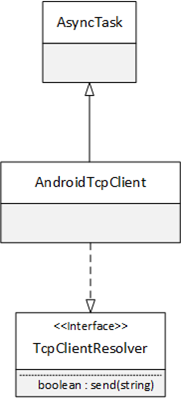
\includegraphics{design/figures/tcp-cd.png}
\caption{Android TCP client class diagram.}
\end{figure}

Similar to the GpsResolver class, the Android MainActivity will pass through an AndroidTcpClient that implements the TcpClientResolver interface for the game to make of use of when it needs to transmit data to to the server.
\newpage
\begin{figure}[h!]
\centering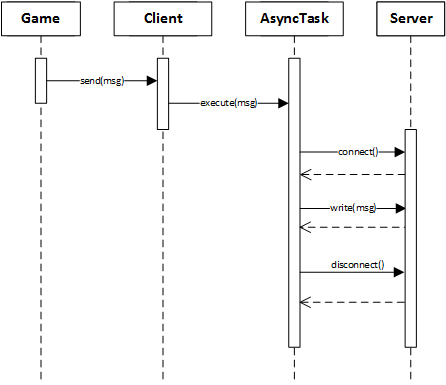
\includegraphics[width=\linewidth]{design/figures/tcp-client-sd.png}
\caption{Android TCP client sequence diagram.}
\end{figure}

The interface exposes the send function to the application to allow it to send data by internally using a class that extends AsyncTask.

\subsubsection{TCP Message Structure}
\label{design:tcp-structure}
Due to this application leaking data by design, the message protocol does not require any encryption and can be relatively simple. There is only one type of message the application needs to send- data. The packet needs to include a uniquely identifiable value for the device that is running the game in order to track users. As it has relatively simple requirements the packet structure will be the packet type- in case of expansion-, device unique identifier followed by the payload. The fields will be delimited by a comma to allow the server to tokenize the packet for processing.

\subsubsection{Unique Identifier}
\label{unique-android-id}
To get a truely unique identifier for a device it would need to be generated on installation of the application. Android helpfully provides an API call to get a somewhat unique number for a device, provided the manufacturer has implemented it. The setting is: 

\begin{verbatim}
Settings.Secure.ANDROID_ID
\end{verbatim}

Although it can be changed if the phone is rooted, or upon factory reset, it is sufficient for this demonstration. The value will need to be added to it's place in the TCP packet when transmiting data.

\subsection{TCP Server}
\label{nodejs}
The TCP server will be incredibly simple as all that is required is the ability for clients to connect and post information to it. Due to this the server will be implemented in node.js as the lines of code it takes to write a a TCP server to this standard is minimal.

\clearpage
\subsection{Requirements Matrix}
This section matches a given requirement from section \ref{requirements:specific} on page \pageref{requirements:specific} with proof that it has been considered in the design. 
\subsubsection{Honeypot Application}
\begin{table}[!h]
	\begin{center}
		\begin{tabular}{ | c |  p{12cm} | }
			\hline
			\textbf{Requirement} & \textbf{Verification} \\ \hline
			1 & The program flow in section \ref{program-flow} details how user defined options are required to create the interface.\\ \hline
			2 & Section \ref{parsing-probe} details how the SSID is captured and compared against the user defined value.\\ \hline
			3 & Capturing and parsing probe requests is detailed in section \ref{parsing-probe}. \\ \hline
			4 & Creating a fake access point is detailed in section \ref{design:create-ap}.\\ \hline
			5 & The TCP client is detailed in section \ref{hp-tcp}.\\ \hline
			6 & Section \ref{open-auth} looks at discovering vulnerable devices that are probing for open authentication networks. \\ \hline
			7 & This is achieved using a bridge tool, which is documented in the implementation.\\ 
			\hline
		\end{tabular}
	\end{center}
\end{table}

\subsubsection{Android Application}
\begin{table}[!h]
	\begin{center}
		\begin{tabular}{ | c |  p{12cm} | }
			\hline
			\textbf{Requirement} & \textbf{Verification} \\ \hline
			1 & Section \ref{design:flappy-bird} describes how the application will be a clone of a popular game.\\ \hline
			2 & The classes required for getting the GPS location are in section \ref{design:ag-lp-cd}.\\ \hline
			3 & This is discussed in section \ref{unique-android-id}.\\ \hline
			4 & Sections \ref{design:ag-tcp-1} and \ref{design:tcp-structure} detail TCP client support. \\ 
			\hline
		\end{tabular}
	\end{center}
\end{table}

\subsubsection{Server Application}
\begin{table}[!h]
	\begin{center}
		\begin{tabular}{ | c |  p{12cm} | }
			\hline
			\textbf{Requirement} & \textbf{Verification} \\ \hline
			1 & The server is discussed in section \ref{nodejs}.\\ \hline
			2 & This requirement is covered in section \ref{nodejs}.\\ 
			\hline
		\end{tabular}
	\end{center}
\end{table}
%%%%%%%%%%%%%%%%%%%%%%%%%%%%%%%%%%%%
\clearpage